%% 
%% Material Suplementar -- Artigo 2
%% Vulnerabilidade biocultural em Saberes Agrícolas Tradicionais
%%

\documentclass[12pt,a4paper]{article}

%% Pacotes
\usepackage{amssymb}
\usepackage{amsmath}
\usepackage{bm}
\usepackage[utf8]{inputenc}
\usepackage[T1]{fontenc}
\usepackage{booktabs}
\usepackage{graphicx}
\graphicspath{{../../}}
\usepackage{float}
\usepackage{hyperref}
\usepackage{natbib}
\usepackage{geometry}
\geometry{margin=2.5cm}
\usepackage{setspace}
\onehalfspacing

\begin{document}

\title{Material Suplementar\\[0.5em]
\large Vulnerabilidade biocultural em Saberes Agrícolas Tradicionais: uma meta-análise quantitativa}

\author{Catuxe Varjão de Santana Oliveira \and Luiz Diego Vidal Santos}

\date{}
\maketitle

\tableofcontents
\newpage

%% ============================================================
%% S1. Diagrama de fluxo PRISMA
%% ============================================================
\section{Diagrama de fluxo PRISMA}
\label{app:prisma}

\begin{figure}[H]
\centering
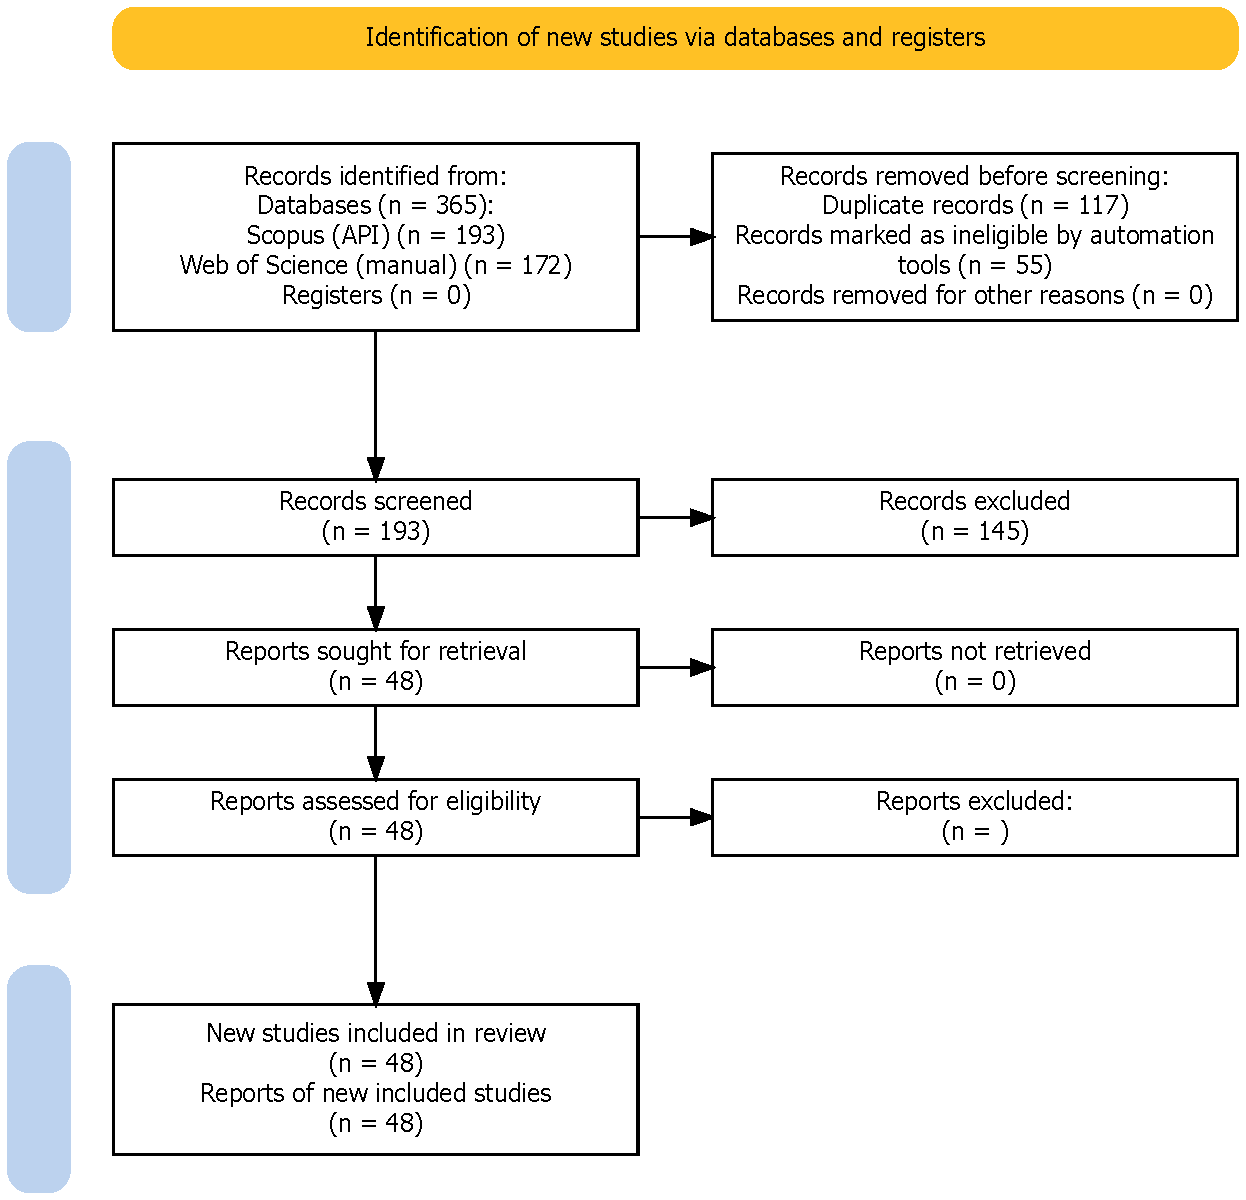
\includegraphics[width=0.88\textwidth]{3-FIGURAS/prisma_flowdiagram_artigo2_en.pdf}
\caption{Diagrama de fluxo PRISMA 2020 mapeando a busca sistemática nas bases Scopus e Web of Science Core Collection, restrições de triagem e a deduplicação entre bancos de dados.}
\label{fig:prisma-flow}
\end{figure}

\newpage

%% ============================================================
%% S2. Resultados da meta-análise por dimensão
%% ============================================================
\section{Resultados da meta-análise por dimensão}
\label{app:tabela}

\begin{table}[H]
\caption{Resultados da meta-análise por dimensão de vulnerabilidade biocultural ($k = 37$ estudos por dimensão, modelo \texttt{rma.mv} com REML e RVE-CR2, $\rho = 0{,}8$).}
\label{tab:meta-results}
\centering
\small
\begin{tabular}{lrrrrrr}
\toprule
\textbf{Dimensão} & $\overline{lnRR}$ & \textbf{EP} & \textbf{IC 95\%} & $\tau^2$ & $I^2$ (\%) & \textbf{Var. \%} \\
\midrule
$V_1$ Eros\~ao Intergeracional    & $-0{,}017$ & 0,108 & $[-0{,}24;\; 0{,}21]$ & 0,169 & 14,8 & $-1{,}7$ \\
$V_2$ Complexidade Biocultural    & $+0{,}045$ & 0,051 & $[-0{,}07;\; 0{,}16]$ & 0,021 &  2,4 & $+4{,}6$ \\
$V_3$ Singularidade Territorial   & $+0{,}072$ & 0,074 & $[-0{,}09;\; 0{,}23]$ & 0,028 &  6,1 & $+7{,}4$ \\
$V_4$ Status de Documenta\c{c}\~ao    & $+0{,}007$ & 0,102 & $[-0{,}21;\; 0{,}22]$ & 0,093 &  7,6 & $+0{,}7$ \\
\textbf{$V_5$ Vulnerabilidade Jur\'idica} & $\mathbf{-0{,}279}$ & \textbf{0,105} & $\mathbf{[-0{,}49;\; -0{,}06]}$ & \textbf{0,171} & \textbf{30,7} & $\mathbf{-24{,}3}$ \\
$V_6$ Organiza\c{c}\~ao Social       & $+0{,}172$ & 0,106 & $[-0{,}05;\; 0{,}40]$ & 0,101 &  8,4 & $+18{,}7$ \\
\bottomrule
\end{tabular}
\begin{flushleft}
\footnotesize \textit{Notas:} EP = erro-padrão robusto (CR2). Var.~\% = $(e^{lnRR} - 1) \times 100$.  IC em negrito indica $p < 0{,}05$.
\end{flushleft}
\end{table}

\newpage

%% ============================================================
%% S3. Mapeamento indicadores-dimensões
%% ============================================================
\section{Mapeamento indicadores-dimensões}
\label{app:mapping}

\begin{table}[H]
\caption{Mapeamento entre indicadores meta-analíticos e dimensões funcionais de vulnerabilidade biocultural.}
\label{tab:mapping}
\centering
\small
\begin{tabular}{p{0.8cm}p{2.0cm}p{3.5cm}p{2.5cm}p{3.0cm}}
\toprule
\textbf{Dim.} & \textbf{Denominação} & \textbf{Indicador meta-analítico ($lnRR$)} & \textbf{Variável funcional} & \textbf{Status de evidência} \\
\midrule
$V_1$ & Erosão Interg. & $\overline{lnRR}_{V_1}$, IC~95\% & Risco de descontinuidade de transmissão & Confirmatório ($k = 37$) \\
$V_2$ & Complexidade & $\overline{lnRR}_{V_2}$, IC~95\% & Densidade biocultural & Confirmatório ($k = 37$) \\
$V_3$ & Singularidade & $\overline{lnRR}_{V_3}$, IC~95\% & Exclusividade territorial & Confirmatório ($k = 37$); base Tier~1 restrita \\
$V_4$ & Documentação & $\overline{lnRR}_{V_4}$, IC~95\% & Grau de registro formal & Confirmatório ($k = 37$); moderadores contextuais \\
$V_5$ & Vuln. Jurídica & $\overline{lnRR}_{V_5}$, IC~95\% & Exposição a apropriação indevida & Confirmatório ($k = 37$); base Tier~1 restrita \\
$V_6$ & Org. Social & $\overline{lnRR}_{V_6}$, IC~95\% & Vitalidade organizacional & Confirmatório ($k = 37$) \\
\bottomrule
\end{tabular}
\end{table}

\newpage

%% ============================================================
%% S4. Diagnóstico de disponibilidade de evidência
%% ============================================================
\section{Diagnóstico de disponibilidade de evidência}
\label{app:viability}

\begin{table}[H]
\caption{Diagnóstico de disponibilidade de evidência e estratégia analítica por dimensão de vulnerabilidade.}
\label{tab:viability}
\centering
\small
\begin{tabular}{p{0.8cm}p{2.2cm}p{1.2cm}p{2.0cm}p{5.5cm}}
\toprule
\textbf{Dim.} & \textbf{Denominação} & \textbf{$k$} & \textbf{Status} & \textbf{Estratégia analítica} \\
\midrule
$V_1$ & Erosão Interg. & 37 & Confirmatória & Meta-análise completa (forest plot, meta-regressão, viés de publicação) \\
$V_2$ & Complexidade & 37 & Confirmatória & Meta-análise completa \\
$V_3$ & Singularidade & 37 & Confirmatória & Meta-análise completa; base Tier~1 restrita, interpretar com cautela \\
$V_4$ & Documentação & 37 & Confirmatória & Meta-análise completa; meta-regressão com moderadores \\
$V_5$ & Vuln. Jurídica & 37 & Confirmatória & Meta-análise completa; base Tier~1 restrita, interpretar com cautela \\
$V_6$ & Org. Social & 37 & Confirmatória & Meta-análise completa; meta-regressão com moderadores \\
\bottomrule
\end{tabular}
\end{table}

\end{document}
